\section{フォトリフレクタ}
\subsection{使用目的}
フォトリフレクタはロボカーがコースのコントロールラインを読み取るために使用する.本研究室では\refig{photosensor}に示す1RC Reflectance Sensorを用いた.このフォトリフレクタを採用した理由は以下で説明する原理よりAD変換器を使用せずGPIOのディジタル入出力のみで利用可能であるためである.   


\subsection{原理}
このフォトリフレクタの内部の回路図\cite{pololu}を\refig{phses_cir}に示す.はじめにRaspberry Pi mobel BのGPIOピンを出力にした後HIGHを出力し回路内のコンデンサを10マイクロ秒充電する.その後先ほどのGPIOピンを入力に変換する.\\
回路内のLEDが対象物に照射した光の反射光がフォトダイオードに入射することによりフォトダイオードに電流が流れるようになりコンデンサの電圧が減衰する.\\
採用したフォトリフレクタ基板はコンデンサの電圧が一定値より大きければHIGH,小さければLOWという二値出力をするような回路が組み込まれているためパルス幅が長ければコンデンサの電圧減衰時間が長いとみなせる.\\
反射光の反射率が大きければコンデンサの電圧減衰時間が短くなり,反射率が小さければコンデンサの電圧減衰時間が長くなるためパルス波のHIGHの幅の長さにより反射率の大きさを測定することができる.\\
反射率の大きさは色によって異なるのでコンデンサの電圧減衰時間,即ちパルス幅を計測することで対象物の色を判別することができる.

\subsection*{仕様}
\begin{itemize}
\item 作動電圧:5.0[V]
\item 電流電源:17[mA]
\item 最適な検出距離:3.0[mm]
\item 最大検出距離:9.5[mm]
\end{itemize}


\subsection{動作確認実験}
\begin{description}
      \item[色判別] \mbox{} \\
      白色の物体と黒色の物体の表面をフォトレフレクタの3mm上にかざし,物体の色を判別できるか実験した.      
      \item[結果] \mbox{} \\
      色判別の実験において正しく白色の物体と黒色の物体を区別することができた.    
\end{description}

\subsection{今後の実験}
\begin{enumerate}

	\item 実際のコースとコントロールラインの色を判別するために各色のフォトリフレクタが出力するパルス幅について閾値を設定し各色の判定をできるようにする.
	
	\item ロボカーが走行しながらコントロールラインを通過した回数を判定できるようにする.

\end{enumerate}

\begin{figure}[htb]
  \centering
    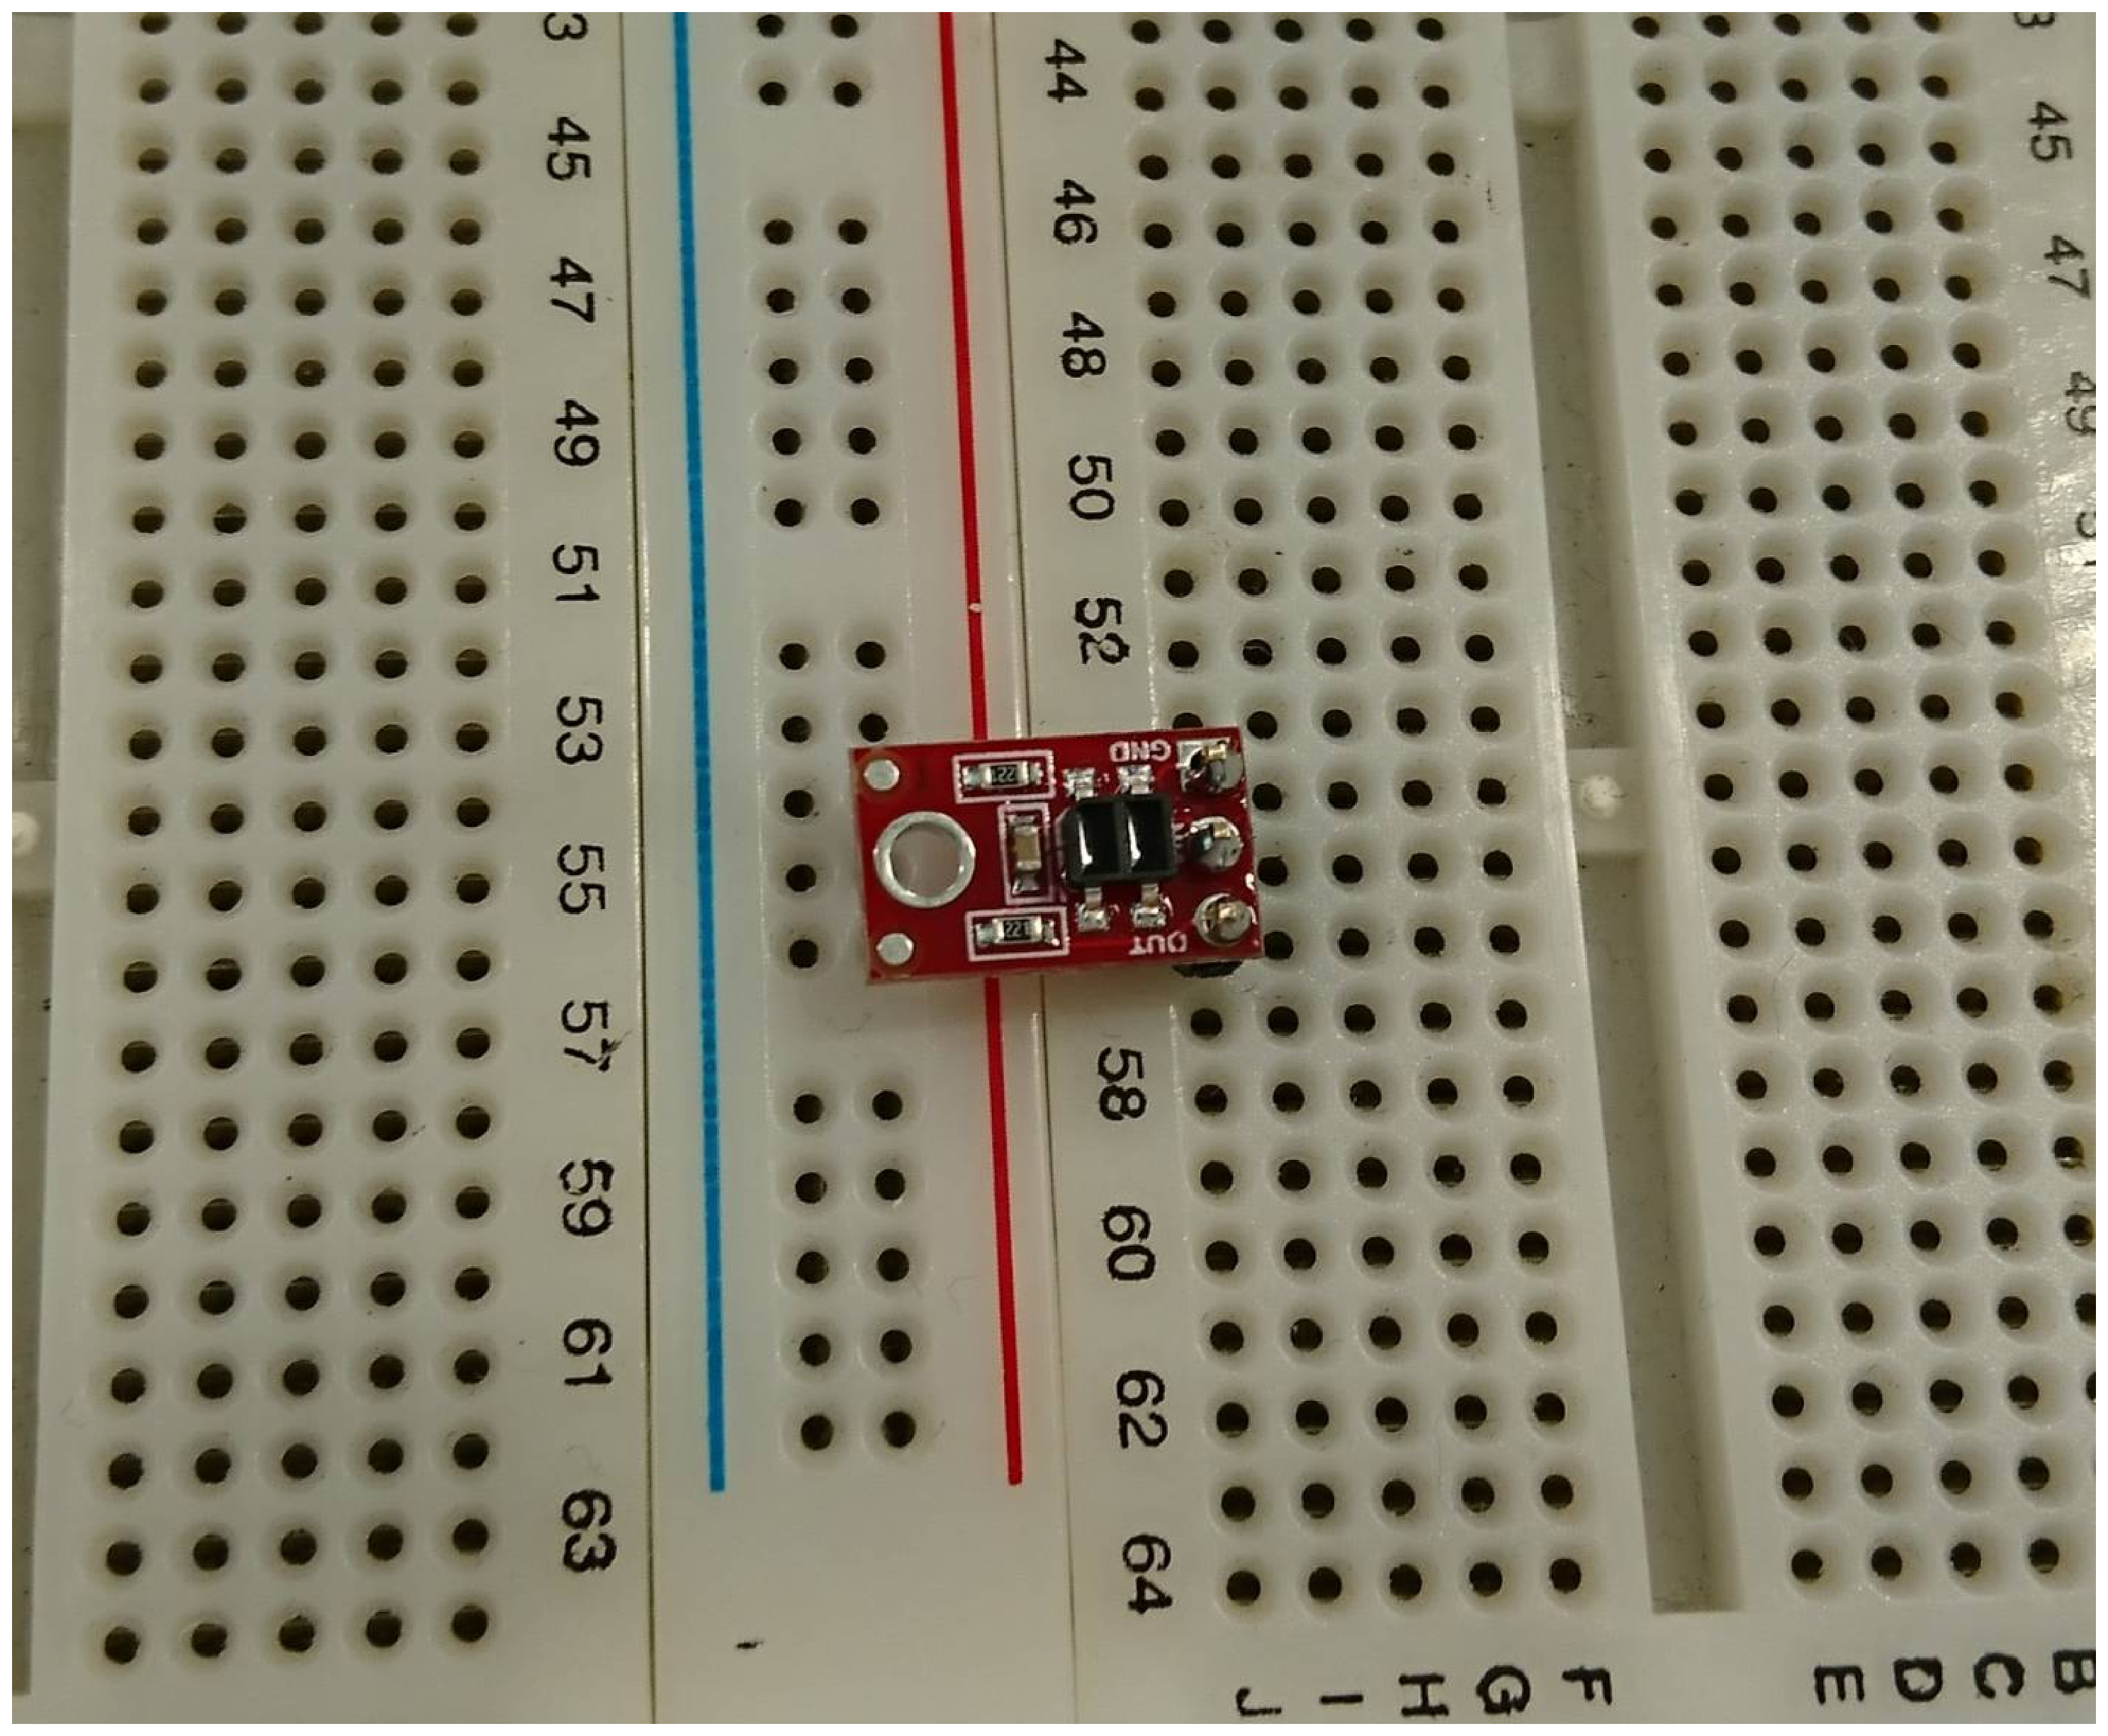
\includegraphics[width=0.5\hsize]{picture/eps/photosensor.eps}
    \caption{フォトリフレクタ}
    \label{fig::photosensor}
\end{figure}

\begin{figure}[htb]
  \centering
    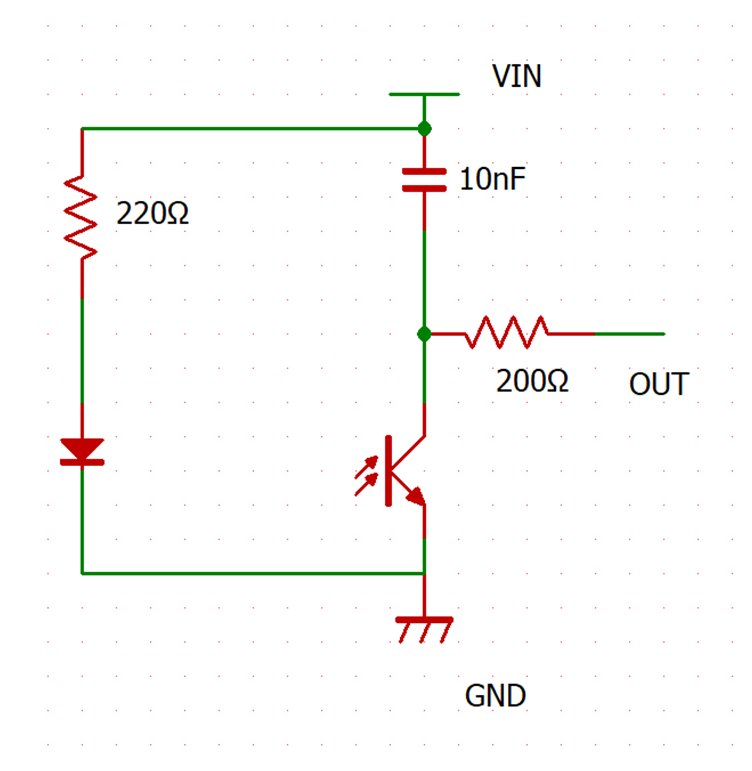
\includegraphics[width=0.5\hsize]{picture/eps/photosensor_circit.eps}
    \caption{フォトリフレクタの内部の回路図}
    \label{fig::phses_cir}
\end{figure}